\documentclass{zc-ust-hw}

\usepackage[]{lipsum} 

\name{SalahDin Ahmed Salh Rezk}
\id{202201079}
\course{Thermodynamics, Wave Motion and Optics}
\assignment{Assignment 10}

\usepackage{import}
\usepackage{xifthen}
\usepackage{pdfpages}

\newcommand{\incfig}[1]{%
    \def\svgwidth{\columnwidth}
    \import{./figures/}{#1.pdf_tex}
}

\begin{document}

\maketitle

\begin{enumerate}
  \item The Figure below shows a hypothetical speed distribution for a sample
    of $N$ gas particles.
    \begin{figure}[htpb]
      \begin{center}
        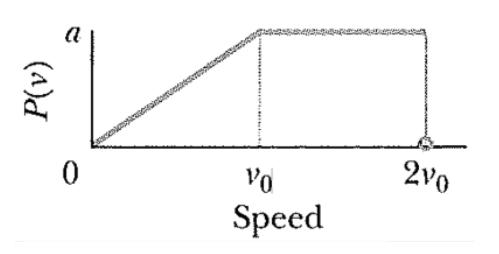
\includegraphics[width=0.45\textwidth]{figures/1705953512.png}
      \end{center}
      \caption{}
    \end{figure}
    
    Let $P(v) = 0$ for speed $v > 2v_o$. What are the values of
    \begin{enumerate}
      \item $a*v_o$
        \begin{sol}
          \begin{align}
            \int P(v)dv &= 1 \\
            &= \frac{1}{2}av_{0}+av_{0} = \frac{3}{2}av_{0} \\
            \frac{3}{2}av_{0} &= 1 \\
            av_{0} &= \frac{2}{3}
          \end{align}
        \end{sol}
      \item $v_{\text{avg}}/v_o$
        \begin{sol}
          \begin{align}
            v_{\text{avg}}&=\int vP(v)dv \\
            \intertext{For the triangular portion \( P(v)=\frac{av}{v_{0}} \):}
            v_{\text{avg\_tri}}&= \frac{a}{v_{0}}\int_{0}^{v_{0}} v^2dv \\
            &= \frac{a}{3v_{0}}v_{0}^3  \\
            &= \frac{av_{0}^2}{3} \\
            \intertext{Use \( av_{0} = \frac{2}{3} \):}
            &= \frac{2}{9}v_{0} \\
            \intertext{For the rectangular portion \( P(v)=av \):}
            v_{\text{avg\_rec}} &= a\int_{v_{0}}^{2v_{0}} vdv  \\
            &= \frac{a}{2}\left( 4v_{0}^2-v_{0}^2 \right)  \\
            &= \frac{3a}{2}v_{0}2 = v_{0} \\
            \intertext{Substituting:}
            v_{\text{avg}}&=\frac{2}{9}v_{0}+v_{0} = \frac{11}{9}v_{0} \\
            \frac{v_{\text{avg}}}{v_{0}} = \frac{11}{9}
          \end{align}
        \end{sol}
      \item $v_{\text{rms}}/v_o$
        \begin{sol}
          \begin{align}
            v_\text{rms} &= \sqrt{\int v^2P(v)dv} \\
             &= \sqrt{\frac{a}{v_{0}}\int_{0}^{v_{0}}v^3 dv+a\int_{v_{0}}^{2v_{0}} v^2dv} \\
             &= \sqrt{\frac{1}{6}v_{0}^2+\frac{14}{9}v_{0}^2}  \\
             &= \sqrt{\frac{31}{18}v_{0}^2}  \\
             &= \frac{\sqrt{62} }{6}v_{0} \\
             \frac{v_\text{rms}}{v_{0}} &= \frac{\sqrt{62} }{6}
          \end{align}
        \end{sol}
      \item What fraction of the particles has a speed between $1.5v_o$ and $2.0v_o$?
        \begin{sol}
          \begin{gather}
            N\int_{1.5v_{0}}^{2v_{0}} P(v)\,dv \\
            \intertext{Using \( P(v)=a \) in the range:}
            Na(2.0v_{0}-1.5v_{0}) = 0.5Nav_{0} = \frac{N}{3}
          \end{gather}
          The fraction of particles in this range is \( \dfrac{1}{3} \).
        \end{sol}
    \end{enumerate}
    
  \item Consider a system of one particle with 128 possible discrete locations
    in space. Assuming that all locations are equally probable:
    \begin{enumerate}
      \item Determine the lack of information in bits
        \begin{sol}
          \begin{align}
            S &= -\Sigma p_i \log_2 p_i \\
            \intertext{Using \( p_i = \frac{1}{128} \)}
            S&=-\Sigma \frac{1}{128}\log_{2}\left( \frac{1}{128} \right) = 7 \\
            127&=2^{6}+2^{5}+2^{4}+2^{3}+2^{2}+2^{1}+2^{0}
          \end{align}
          Therefore if all digits are zeros, the particle resides in the state 128.
        \end{sol}
      \item What if you know that 64 of which are forbidden states for the particle?
        \begin{sol}
          \begin{align}
            S&=-\Sigma \frac{1}{64}\log_{2}\left( \frac{1}{64} \right) = 6 \\
            63&=2^{5}+2^{4}+2^{3}+2^{2}+2^{1}+2^{0}
          \end{align}
        \end{sol}
    \end{enumerate}
    
  \item An isolated Thermos contains 130 g of water at 80 \textdegree C. You
    put in a 12 g ice cube at 0 \textdegree C to form a system of ice + original
    water ($L_f = 333\times 10^3$ J/Kg, c = 4190 J/(Kg.C))
    \begin{enumerate}
      \item What is the equilibrium temperature of the system?
        \begin{sol}
          \begin{gather}
            \Sigma Q=0 \implies L_fm+cm(T_f-0)+cm'(T_f-80)=0 \\
            \intertext{Substituting values:}
            T_f = 339.67 \text{ K}
          \end{gather}
        \end{sol}
      \item What are the entropy changes of the water that was originally the
        ice cube as it melts? and
        \begin{sol}
          \begin{equation}
            \frac{Q}{T} = \frac{L_fm}{273.15} = 14.6 \text{ J/K}
          \end{equation}
        \end{sol}
      \item as it warms to the equilibrium temperature?
        \begin{sol}
          \begin{equation}
            \int_{273.15}^{339.67} \frac{cm}{T}\,dT=cm \ln \left(\frac{339.67}{273.15}\right) = 11.0 \text{ J/K}
          \end{equation}
        \end{sol}
      \item What is the entropy change of the original water as it cools to the
        equilibrium temperature?
        \begin{sol}
          \begin{equation}
            \int_{353.15}^{339.67} \frac{cm'}{T}dT = cm'\ln \left( \frac{339.67}{353.15} \right)  = -21.2 \text{ J/K}
          \end{equation}
        \end{sol}
      \item What is the net entropy change of the ice + original water system
        as it reaches the equilibrium temperature?
        \begin{sol}
          \begin{equation}
            \Delta S_\text{net} = 14.6 + 11.0 - 21.2 = 4.39 \text{ J/K}
          \end{equation}
        \end{sol}
  \end{enumerate}

\item A multi-cylinder gasoline engine in an airplane, operating at 2500
  rev/min, takes in energy $7.89 \times  10^3$ J and exhausts $4.58 \times 10^3$ J for each
  revolution of the crankshaft.  

  \begin{enumerate}
    \item How many liters of fuel does it consume in 1.0 h of operation if the
      heat of combustion is $4.03\times 10^7$ J/L?  
      \begin{sol}
        \begin{align}
          7.89\times 10^3 \cdot 2500 \times \frac{60}{1} &= 1.18 \times 10^9 \text{ J/h} \\
          \frac{1.18\times 10^{9} }{4.03\times 10^{7} } &= 29.4 \text{ L/h}
        .\end{align}
      \end{sol}
    \item What is the mechanical power output of the engine? Ignore friction.
      \begin{sol}
        \begin{align}
          W_\text{eng} &= Q_h - Q_c \\
          \frac{W_\text{eng}}{dt} &= \frac{Q_h}{dt} - \frac{Q_c}{dt} \\
          &= \left( 7.89\times 10^3 -4.58\times 10^3  \right) \cdot \frac{2500}{60} \\
          &= 1.38 \times 10^{5} \text{ W} 
        .\end{align}
      \end{sol}
    \item What power must the exhaust and cooling system transfer out of the engine?
      \begin{sol}
        \begin{equation}
          \frac{Q_c}{dt} = 4.58\times 10^3 \cdot \frac{2500}{60} = 1.91\times 10^{5} \text{ W} 
        .\end{equation}
      \end{sol}
    \item Bonus: What is the torque exerted by the crankshaft on the load?
      \begin{sol}
        \begin{equation}
          \tau = \frac{W_\text{eng} }{\omega }= \frac{1.38\times 10^{5} }{2500 /60}\cdot \frac{1}{2\pi } = 527 \text{ N.m}
        .\end{equation}
      \end{sol}
  \end{enumerate}

\item Suppose a heat engine working with a $vdW$ gas with a known constant $b$
  and a temperature-independent heat capacity $c_V$. If the gas undergoes a
  cycle that consists of two isochors ($V_1$ and $V_2$) and two adiabats
  processes. Deduce the efficiency of the heat engine.
  \begin{sol}
    \begin{align}
      e &= 1-\frac{\Delta Q_c}{\Delta Q_h} \\
      &= 1-\frac{T_B-T_C}{T_A-T_D} \\
      S_{vdW}&=\frac{f}{2}Nk_B\ln T+Nk_B\ln (V-Nb)+const \\
      S_{vdW}&=\frac{f}{2}Nk_B\ln \left( \frac{T_f}{T_i} \right) +Nk_B\ln \left( \frac{V_f-Nb}{V_i-Nb} \right) \\
      \intertext{For adiabatic process:}
      0&=\frac{f}{2}Nk_B\ln \left( \frac{T_f}{T_i} \right) +Nk_B\ln \left( \frac{V_f-Nb}{V_i-Nb} \right) \iff T^{\frac{f}{2}}(V-Nb)=const 
      e&=1-\left( \frac{V_1-Nb}{V_2-Nb} \right)^{\frac{R}{c_V}} 
    .\end{align}
  \end{sol}

  \newpage

\item For a Carnot cycle where the working substance is a Van der Waals gas and
  the cycle processes are as shown in Figure 1-2 and 3-4 are isotherms, 2-3 and
  4-1 – adiabats. The temperatures of the hot and cold reservoirs are $T_H$ and
  TC, respectively.

  \begin{enumerate}
    \item Draw the cycle.
      \begin{sol}\end{sol}
      \begin{figure}[H]
        \begin{center}
          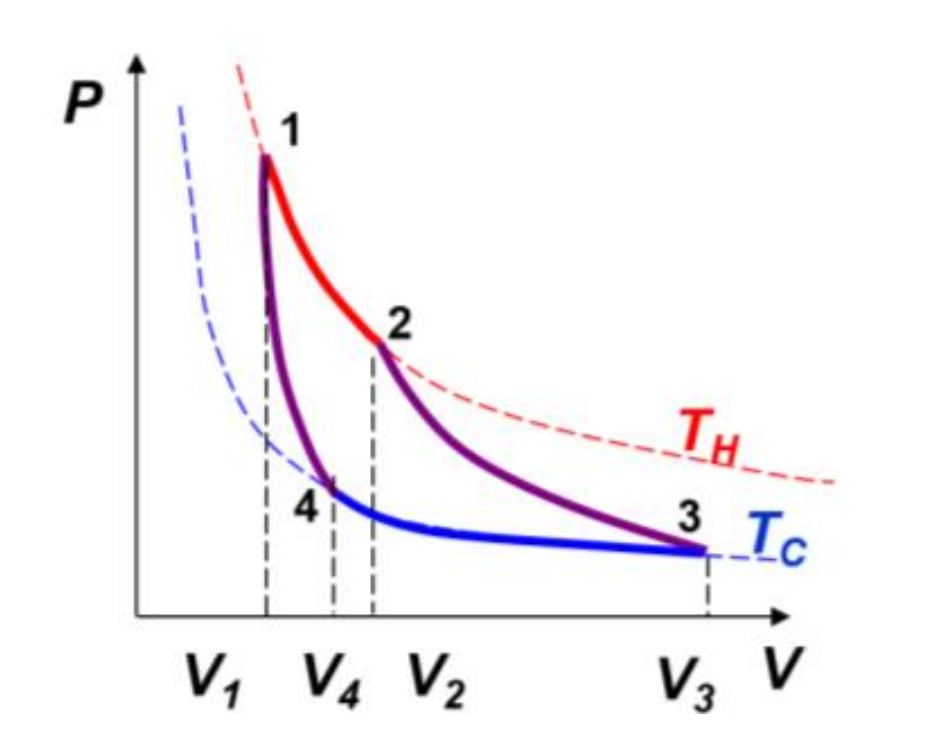
\includegraphics[width=0.5\textwidth]{figures/1705958348.png}
        \end{center}
        \caption{}
      \end{figure}
    \item Deduce the efficiency of this heat engine.
      \begin{sol}
        \begin{align}
          e &= 1-\frac{\Delta Q_c}{\Delta Q_h} \\
          \intertext{1-2 and 3-4 isothermal expansion}
          \Delta U&=\Delta Q+\Delta W \\
          \Delta U_{vdW} |_T &= N^2a(\frac{1}{v_i}-\frac{1}{V_f}) \\
          \Delta W &= -\int_{V_i}^{V_f} (\frac{Nk_BT}{V-Nb}-\frac{N^2a}{V^2}) \, dV \\
                   &= -Nk_bT\ln \left( \frac{V_f-Nb}{V_i-Nb} \right) +N^2a(\frac{1}{V_i}-\frac{1}{V_f}) \\
          \Delta Q_{1-2} &= Nk_BT_H\ln \left( \frac{V_2-Nb}{V_1-Nb} \right) \\
          \Delta Q_{3-4} &= Nk_BT_H\ln \left( \frac{V_2-Nb}{V_1-Nb} \right) \\
          e &= 1 - \frac{T_C\ln \left( \frac{V_3-Nb}{V_4-Nb} \right) }{T_H\ln \left( \frac{V_2-Nb}{V_1-Nb} \right) } \\
          \intertext{2-3 and 4-1 adiabatic and quasistatic}
          \Delta Q &= 0 \\
          \Delta U &= \Delta W \\
          S_{vdW}&=\frac{f}{2}Nk_B\ln T+Nk_B\ln (V-Nb)+const \\
          S_{vdW}&=\frac{f}{2}Nk_B\ln \left( \frac{T_f}{T_i} \right) +Nk_B\ln \left( \frac{V_f-Nb}{V_i-Nb} \right) \\
          \intertext{For adiabatic process:}
          0&=\frac{f}{2}Nk_B\ln \left( \frac{T_f}{T_i} \right) +Nk_B\ln \left( \frac{V_f-Nb}{V_i-Nb} \right) \\
          T^{\frac{f}{2}}(V-Nb)&=const \\
          V_4-Nb&=(V_1-Nb)\left( \frac{T_H}{T_C} \right)^{\frac{f}{2}} \\
          V_3-Nb&=(V_2-Nb)\left( \frac{T_H}{T_C} \right)^{\frac{f}{2}} \\
          e = 1-\frac{T_C}{T_H}
        .\end{align}
      \end{sol}
    \item Compare the result in (b) with that for the Carnot cycle with an ideal gas.
      \begin{sol}
        The same as of the cycle of an ideal gas.
      \end{sol}
  \end{enumerate}

  \newpage

\item Suppose you are given 1 kg of water at temperature 1000C and a block of
  ice at temperature 00C. If a reversible heat engine absorbs heat from the
  water and expels heat to the ice until that point at which work can no longer
  be extracted from the system. Given that the heat capacity of water is 4.2
  J/g·K and the heat of fusion of ice is 333 J/g. When the process is complete: 

  \begin{enumerate}
    \item Calculate the temperature of the water. 
      \begin{sol}
        \begin{align}
          e&= 1-\frac{T_\text{ice}}{T_\text{water}}=0 \\
          T_\text{water} = T_\text{ice} = 0^{\circ}\text{ C} 
        .\end{align}
      \end{sol}
    \item Calculate the heat absorbed by the block of ice in the process. 
      \begin{sol}
        \begin{align}
          e &= 1-\frac{\Delta Q_C}{\Delta Q_H} \\
          Q_C&=\int_{T_i}^{T_f}(1-e)m_wc_wdT=m_wc_w\int_{273}^{373} \frac{273}{T}dT \\
          &= 1 \times 4.2 \times  273 \times \ln \left( \frac{373}{273} \right)  \\
          &= 357.9\text{ kJ} \\
        .\end{align}
      \end{sol}
    \item Deduce how much ice has been melted. 
      \begin{sol}
        \begin{equation}
          M_\text{ice} = \frac{Q_C}{L} = \frac{357.9}{333} = 1.07\text{ kg}
        .\end{equation}
      \end{sol}
    \item Calculate the work done by the engine. 
      \begin{sol}
        \begin{align*}
          W = Q_H - Q_C = 1 \times 4.2 \times 100 -357.9=62.1\text{ kJ}
        .\end{align*}
      \end{sol}
  \end{enumerate}

\end{enumerate}

\end{document}
